\chapter{Spectrum sensing}

Spectrum sensing is the main task in the entire operation of cognitive
radio. Spectrum sensing is defined as the finding of spectrum holes in 
the local neighborhood of the cognitive radio receiver. Spectrum holes are the
underutilized (in part or in full) subbands of spectrum at a particular time
in a specific location. Moreover for cognitive radio to fulfil its potential
in solving the problem of spectrum underutilization, the spectrum sensing 
method used should be reliable and computationally feasible in real-time 
\cite{haykin09}.

There are many spectrum sensing techniques available. Three important ones of
them are as follows:
\begin{itemize}
    \item Energy detection
    \item Matched filter detection
    \item Cyclostationarity detection
\end{itemize}

\section{Energy detection}

Conventional energy detector is made up of a low pass filter, an A/D 
converter, a square law detector and an integrator (Figure 
\ref{energyDetection}a). This implementation is not flexible enough, 
especially in the case of narrowband signals and sinewaves. Also, this 
requires a pre-filter matched to the bandwidth $B$ of the signal to be scanned
\cite{cabric06}.

So, an alternative implementation is generally used where we find the squared 
magnitude of the FFT using the Average Periodogram method (Figure 
\ref{energyDetection}b). In this architecture, we can alter the bandwidth of
frequencies scanned just by taking
the required number of FFT bins. 

Spectrum sensing can be viewed as a binary hypothesis-testing problem 
\cite{zhang09}:
\begin{itemize}
    \item $H0$: primary user is absent
    \item $H1$: primary user is present
\end{itemize}

The detection is basically to decide between the following two hypotheses,
\begin{align}
    x(t) &= n(t), & H0 \nonumber \\
    x(t) &= h(t)s(t) + n(t), & H1 \nonumber
\end{align}

where $x(t)$ is the received signal, $s(t)$ is the primary user signal, $h(t)$
is the complex channel gain and $n(t)$ is the additive white gaussian noise
(AWGN) with zero mean and variance $\sigma_n^2$. Generally $h(t)$ is assumed
to be constant $h_0$ for the detection period. A statistics $Y$ is computed by
taking energy samples over a time $T$ in a bandwidth $B$ and compared with a 
predefined threshold $\gamma$ for making the decision.

Energy detection is one of the simplest methods of spectrum sensing. It is the 
optimal detection method for unknown signals. Moreover, it is widely used 
because its computationally less resource-intensive.

\begin{figure}
    \centering
    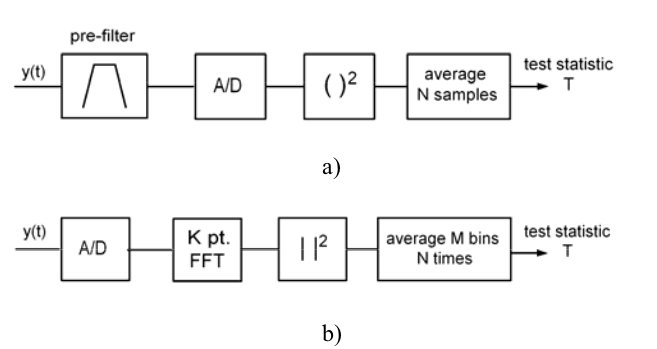
\includegraphics[width=0.7\textwidth]{energyDetection}
    \caption[Energy Detection block diagram]{(a) Implementation using analog 
    filter and square law device \\
    (b) Implementation using periodogram. \\
    \footnotesize{Source: \cite{cabric06}}}
    \label{energyDetection}
\end{figure}

But this method is not without problems. It is always to difficult to 
determine a threshold that will work for all situations. This method cannot
say whether an interfering signal is from a primary user or a secondary user.
Low SNR (signal to noise ratio) signals cannot be detected easily.

The frequency resolution can be improved by increasing N, the number of FFT 
points, but then this requires more samples and thereby takes more time.

\section{Matched filter detection}
A matched filter is a linear filter to maximize the output SNR of a received 
signal. It is the optimum filter to detect signals that are known a priori 
\cite{wikiMF}.


In matched filtering, the received signal is first band pass filtered and then
convolved with the impulse response. The impulse response $h$ here is the 
reference signal itself \cite{bhatta11}. Matched filtering is so called 
because the impulse response is matched to the reference signal.
\begin{equation*}
    Y[n] = \sum_{-\infty}^{\infty} h[n-k]x[k]
\end{equation*}

Here, $x[k]$ is the received or unknown signal with additive noise.
The goal of matched filtering is to enhance the component of reference signal
in the received signal and to suppress the noise. This works best when the 
additive noise is completely orthogonal to the reference signal or when the
noise is completely Gaussian. In practice though, the noise doesn't turn out 
to be purely Gaussian.
 
Matched filtering requires only $O$(1/SNR) samples to meet a given $P_d$, 
probability of detection requirement. Thus it requires less detection time.

But, matched filtering requires us to have a priori information about the 
received signal. This technique requires demodulating the received signal. For
demodulation, we require information like bandwidth, operating frequency, 
modulation type, pulse shaping, packet format, etc. Demodulating the received
signal correctly also requires timing synchronization, carrier 
synchronization, etc. It might still be possible to achive this because the
received data carry preambles, synchronization data, etc.

This method requires a specific type of receiver for every primary user.
Implementing this method on a receiver will increase the complexity and the 
power consumption greatly.

\begin{figure}
\centering
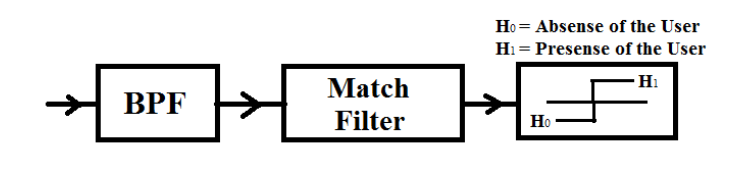
\includegraphics[width=0.8\textwidth]{matchedFilter}
\caption[Matched filter]{Block diagram of Matched filter implementation.}
\label{matchedFilter}
\end{figure}

\section{Cyclostationarity detection}


